\documentclass[aspectratio=169]{beamer}
\beamertemplatenavigationsymbolsempty
\setbeamertemplate{footline}{% 
  \hfill% 
  \usebeamercolor[fg]{page number in head/foot}% 
  \usebeamerfont{page number in head/foot}% 
  \insertframenumber\,%
  %\,/\,\inserttotalframenumber
  \kern1em\vskip5pt% 
}
\usepackage[utf8]{inputenc}
\definecolor{UniBlue}{RGB}{0,0,200}
\setbeamercolor{title}{fg=UniBlue}
\setbeamercolor{frametitle}{fg=UniBlue}
\setbeamercolor{structure}{fg=UniBlue}
\usepackage{graphics}
\usepackage{amsmath}
\usepackage{pgfplots,tikz}
\usetikzlibrary{external,arrows.meta,calc,shapes,pgfplots.groupplots,decorations.markings,graphs,spy,intersections, backgrounds}
% \tikzexternalize[prefix=tikzFiles/]
\DeclareMathOperator*{\argmin}{arg\,min}
\DeclareMathOperator*{\argmax}{arg\,max}
\title{Ideas for Plotting}
\author{Paul Schwerdtner}
\date{September 14, 2021 \\\vspace{1cm} \texttt{schwerdt@math.tu-berlin.de} \\\vspace{1cm} GAMM-Juniors Fall Meeting}
\begin{document}
\begin{frame}[plain] % 
  \addtocounter{framenumber}{-1}
  \maketitle
\end{frame}

\begin{frame} % A stochastic process
    \frametitle{A stochastic process I}
    \centering
    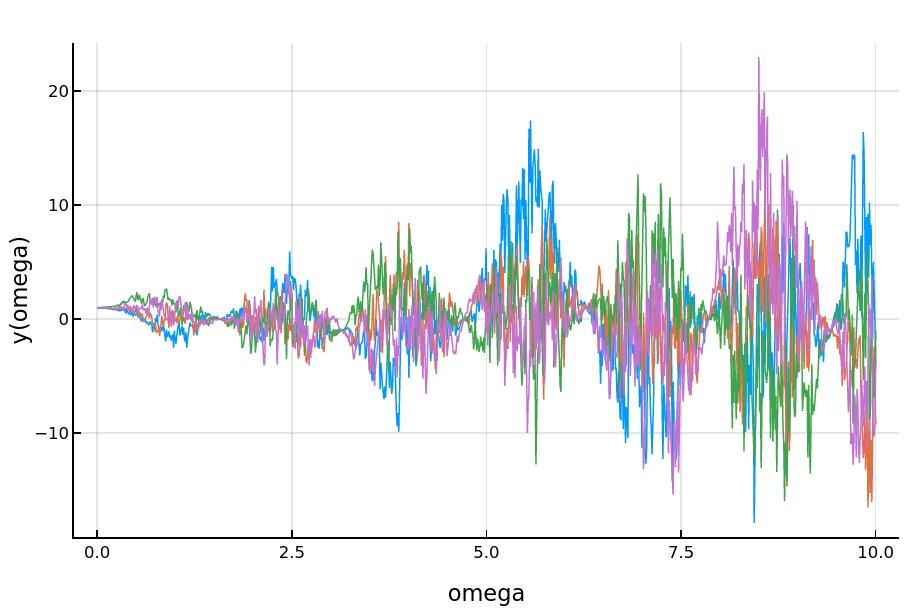
\includegraphics[width=0.8\textwidth]{./PlotSources/terrible.jpg}
\end{frame}

\begin{frame} % A stochastic process
    \frametitle{A stochastic process II}
    \centering
    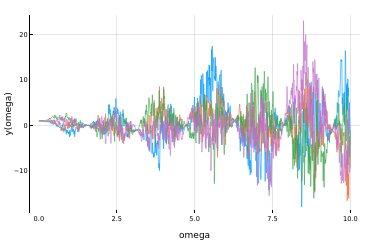
\includegraphics[width=0.8\textwidth]{./PlotSources/more_terrible.jpg}
\end{frame}

\begin{frame} % A stochastic process
    \frametitle{A stochastic process III}
    \centering
    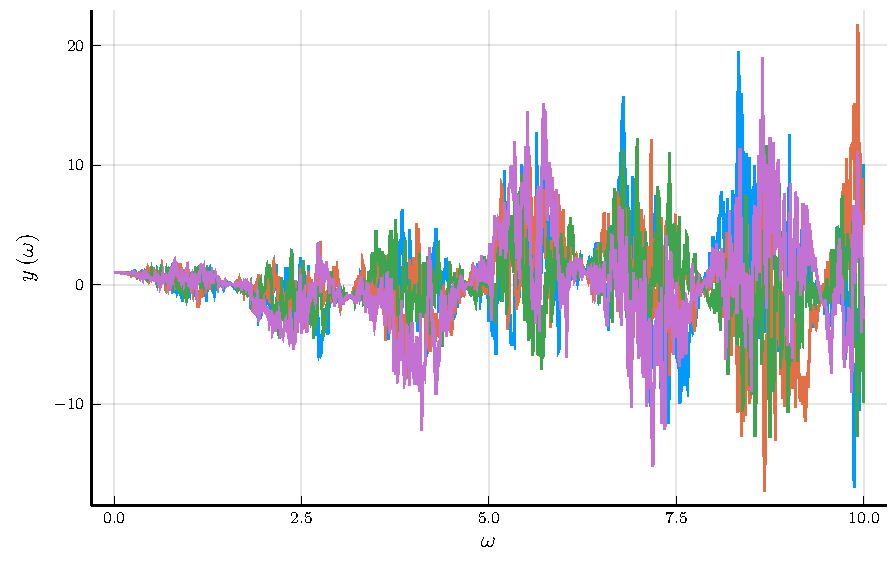
\includegraphics[width=0.8\textwidth]{./PlotSources/less_terrible.pdf}
\end{frame}

\begin{frame} % A stochastic process
    \frametitle{A stochastic process IV}
    \centering
    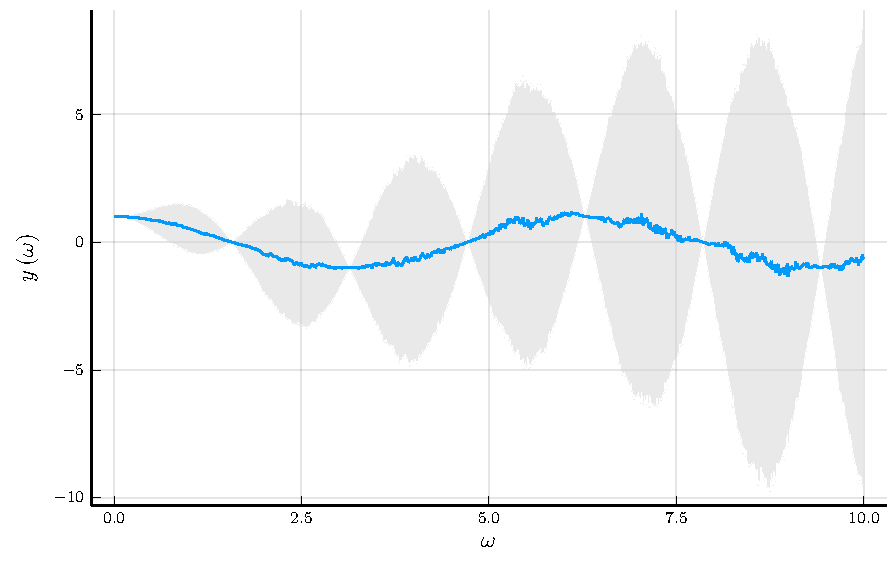
\includegraphics[width=0.8\textwidth]{./PlotSources/std1.pdf}
\end{frame}

\begin{frame} % A stochastic process
  \frametitle{A problem description}
    \centering
    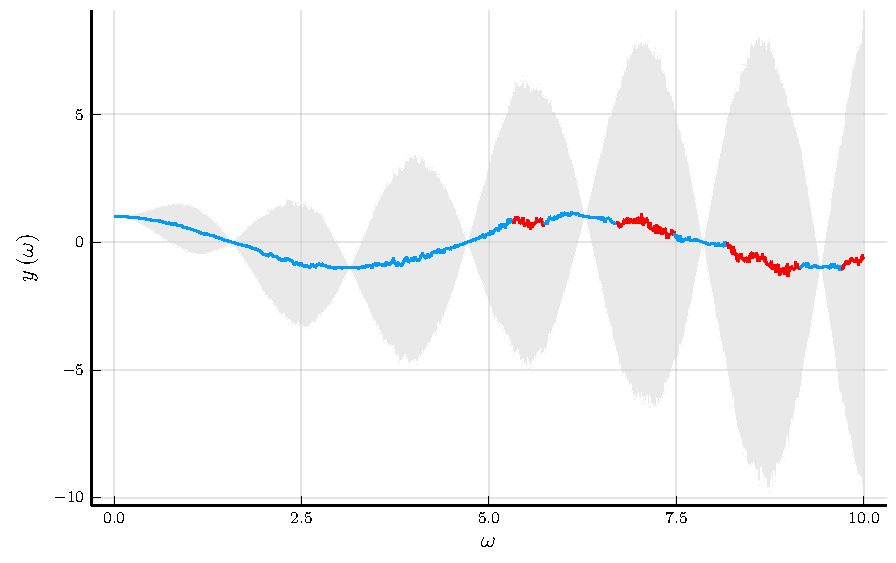
\includegraphics[width=0.8\textwidth]{./PlotSources/std2.pdf}
\end{frame}

\begin{frame} % A stochastic process
  \frametitle{A problem description}
    \centering
    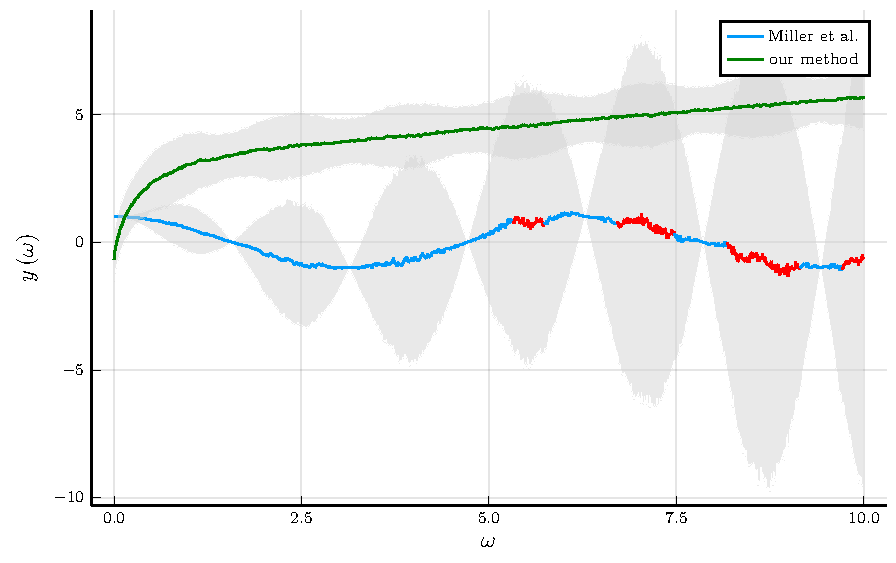
\includegraphics[width=0.8\textwidth]{./PlotSources/std3.pdf}
\end{frame}

\begin{frame} % A stochastic process
  \frametitle{A scientific result}
    \centering
    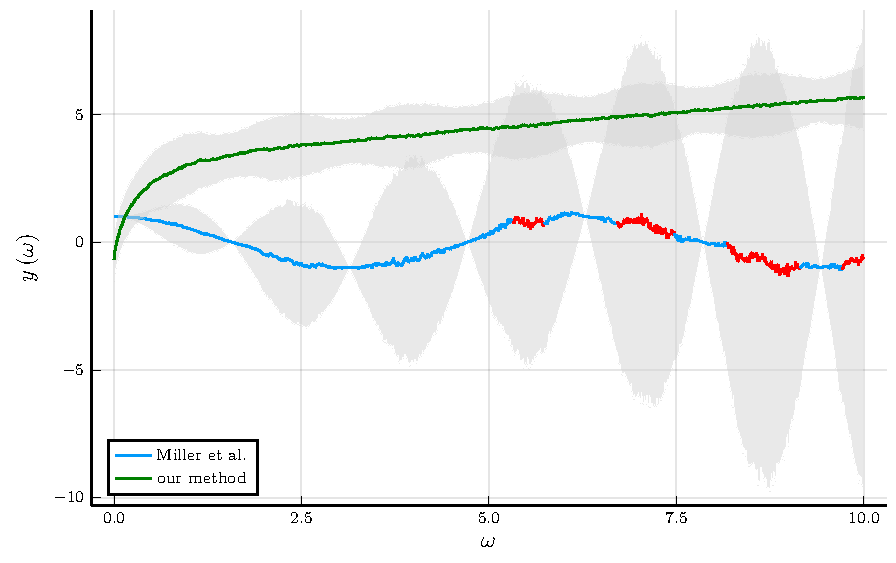
\includegraphics[width=0.8\textwidth]{./PlotSources/std4.pdf}
\end{frame}



\end{document}
